\chapter{Море Киян}

У меня в голове давно бродила шальная мысль, что возле Киева когда-то было море. Его упоминают и  старинные заклинания, что начинаются с убаюкивающей присказки – на море-окияне...

Когда я обратился к сборникам русских заклинаний и шептаний\footnote{В известных мне публикациях украинских заклинаний тоже встречается запев «на морі», но уже на «окіяні», остров Буян, дуб, но камень «білорізь».}, то обнаружил там более четкое название этого моря – в половине случаев говорится не «Окиян», а «Киян». На море на Кияне. Далее следует примерно такое – на острове на Буяне (Кургане)\footnote{Буян по корню сходно со словами «буево» – кладбище, «буйвище» – место прежнего кладбища. Вероятно и Буян означает нечто погребальное, вроде Могильного Острова. На это указывает и замена названия «Буяна» на «Курган».}, стоит бел-горюч камень Алатырь (Латырь). 

Алатырь или Латырь это янтарь. В некоторых – пермских краев – заговорах, вместо Алатырь так и говорится – Янтарь. Однако ведь янтарь желтоватый, верно? Но в старину белым обозначали чистое, светлое, прозрачное. Янтарь можно назвать и белым. Учтем, что значения названий основных цветов сейчас вообще трудно восстановить. Возможно, коричневый – от коры. Красный – красивый. Зеленый – наверное от слова «зело». А черный? Вот шоры лошадям на глаза надевали, но что значат эти «шоры» – тьму? А синий? А желтый? Желтый кстати смахивает на английское «gold». Если букву «g» читать как «ж», а не «г», то получится «жолд», что близко к «желтому».

Так вот об янтаре. На берегу нынешнего Киевского моря, около Межигорья, на холмах у поселка Новые Петровцы, попадается янтарь. Об этом упоминал еще в 19 веке Похилевич в своих «Сказаниях о населенных местностях»:

\begin{quotation}
село расположено на возвышенностях вокруг Межигорья; названо Новыми Петровцами в отличие от Старых, в 3-х верстах выше по Днепру лежащих. Основание Новых Петровец должно относить ко времени наибольшего процветания Межигорского монастыря, когда ему встретилась нужда иметь готовую прислугу под рукой, а не обращаться за ней в более или менее отдалённые свои имения. Грамоты королевские, в коих упоминается село Петровцы, относится к Старым Петровцам. [...]

%В настоящее время жителей обоего пола православных 1442, евреев 18. С 1859 года, как сказано выше, Петровцы отчислены из-под ведения фабрики, с предоставлением им входить в добровольные условия с содержателем её в случае снятия каких-либо фабричных работ. Жители также с успехом занимаются хлебопашеством, огородничеством и садоводством, но особенную их промышленность составляет выделка так называемого межигорского кирпича, известного своей огнеупорностью и твёрдостью, равняющейся твёрдости черепка. Он делается меньшего формата, нежели обыкновенный строительный и покупается на постройку печей. В Петровцах делают его до 500 000 штук ежегодно. 

Замечательно, что в горах петровецких попадается часто янтарь.
\end{quotation}

Испокон веков местное население торговало этим янтарем. Генерал-губернатору Бибикову в 1845 году докладывали: «Честь имею донести, что в Межигорье мальчики деревенские находят и продают янтарь целыми кусками». Искали его весной, в оврагах гор, когда оттуда большими обломками вымывались камни янтаря. Кроме как для продажи, он использовался в знахарских целях и для курения. Вот почему «горюч камень».

Был янтарь и в самом Киеве. В статье 1874 года «Исследование формации бурого угля Киевской губернии» Афанасий Рогович отмечает залежи янтаря около кирпичного завода Эйсмана (позже – Субботиной), а это у озера Глинки близ Лыбедской площади. Когда его берега еще не были застроены, я там лазал по обрыву, но ничего не нашел.

Хорошо, но ведь Киевское море – искусственное водохранилище. А как оно образовалось? Плотиной подняли уровень воды, вода заполнила впадину, потопив около трехсот селений. А впадина откуда? Неужели выкопали?

Нет, была издревле. Если перенестись в прошлое и представить, что в некоторое время уровень воды был выше, то получим точное подобие современного Киевского моря.

Оно кстати не такое уж глубокое. Мелководье – полтора метра, половина площади – три метра, есть под семь. Учтем наносы.

\begin{center}
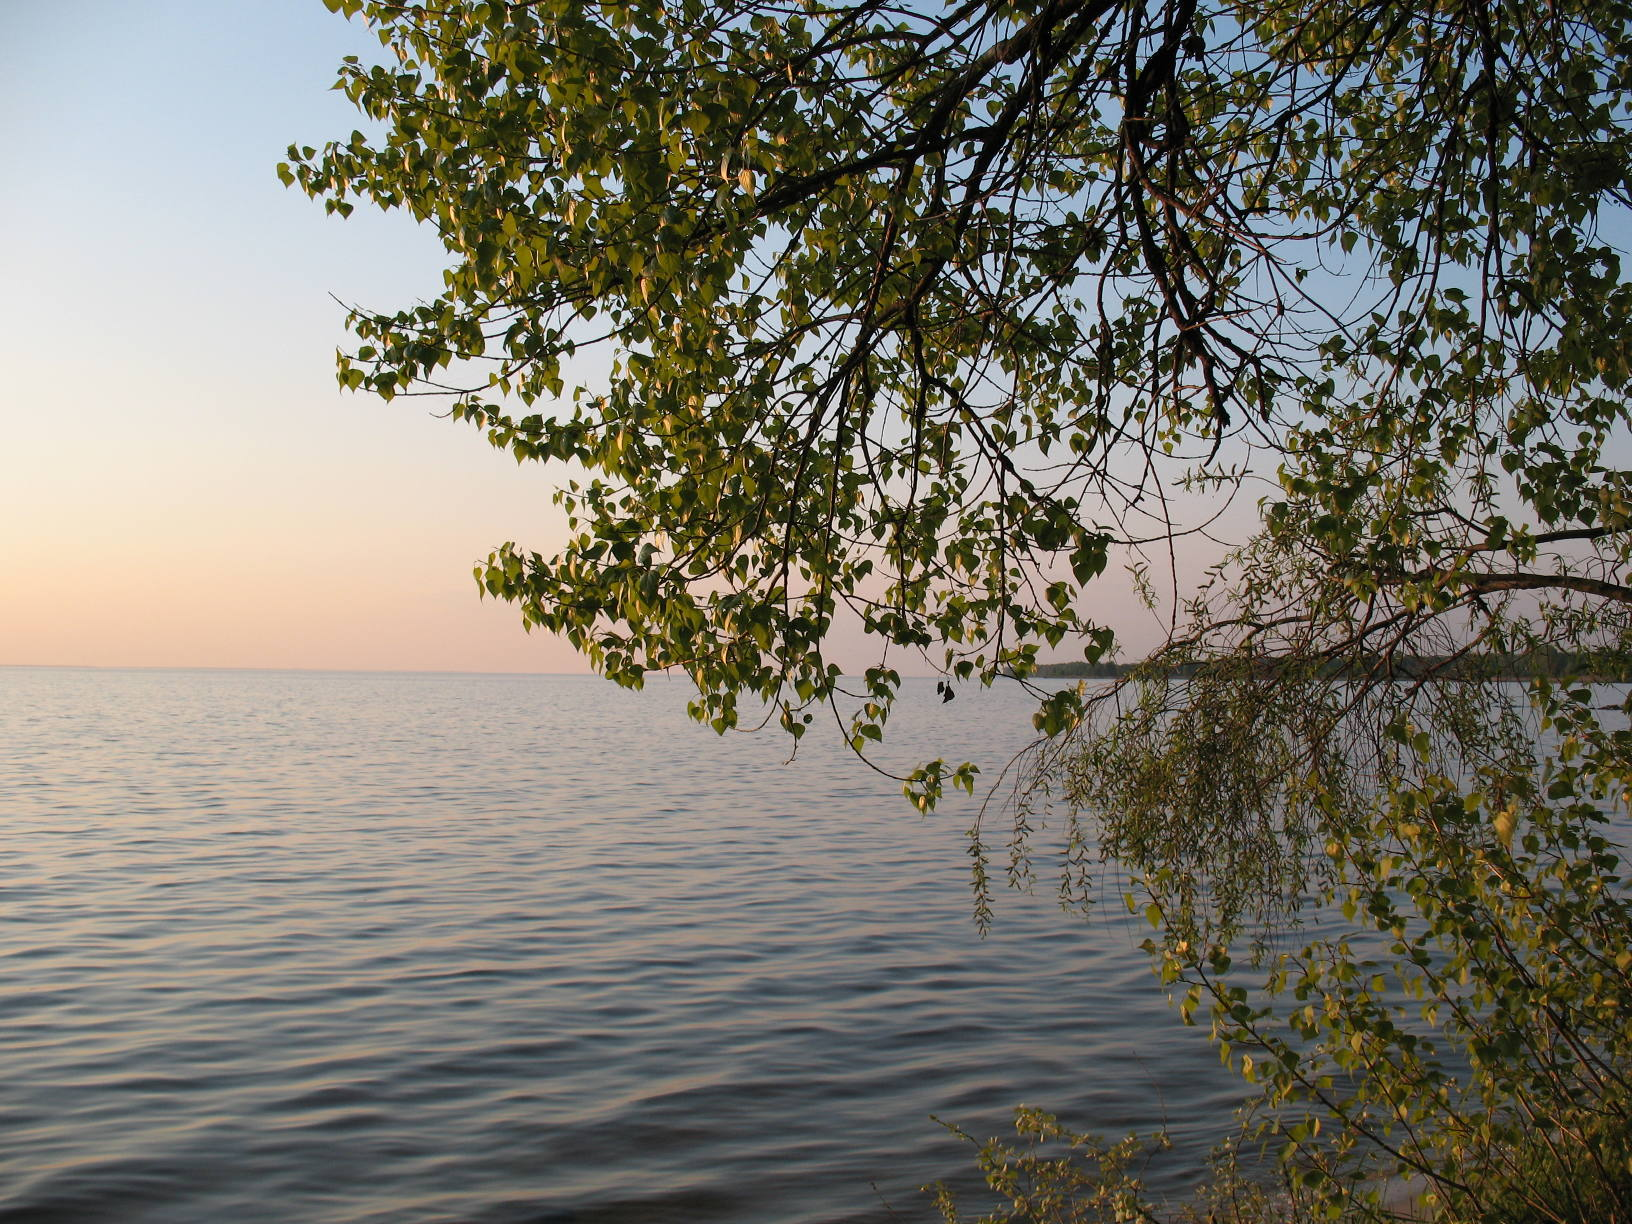
\includegraphics[width=\linewidth]{chast-gorodki/more/s_IMG_0577.jpg}

\textit{Киевское море, 2008 г. Фото Александра Бородина.}
\end{center}

А есть ли острова в этом море? Есть. Пауков\footnote{50°38'43"N 30°30'34"E}. Один из двух уцелевших на месте бывшего тут крупного (с Вышгород) поселка Сваромье, выглядит как плоский луг с лесом. А в северной части моря – Хильча близ дельты Тетерева, Волчьи горы\footnote{51°2'54"N 30°34'16"E}, Длинный, Майорский, Тятин, Прорезные острова, Бакланий и другие. Словом, в седую старину при повышенном уровне воды могло быть и море, и остров Буян или Курган на нем, где находили камень Алатырь – янтарь. Может, остров был священным, ибо заговоры толкуют про дуб на нем.% Не оттуда ли «перуновы дубы», что нашли в Днепре ниже устья Десны?

В первые годы после устроения Киевского водохранилища, площадь островов на нем была 21 км². Постепенно они размывались и остались только перечисленные.
 
В районе Киевского моря, в Днепр впадали и впадают крупнейшие его притоки – Припять, воды которой составляют 27 процентов общего стока Днепра, Десна – 20 процентов общего стока (устье Десны лежит южнее водохранилища на 4 км.), Тетерев – 13 процентов. Больше них только Сож в Белоруси (8,7 процентов), Сула (2,5), Псёл (3,6). Знаменитая Ворскла дает только 1,9 процента общего стока. По числам видно, что именно в районе теперешнего Киевского моря от притоков образуется основной сток Днепра. В море впадают и другие притоки – Ирпень, Козка, Смоловая.

Геологи и гидрологи утверждают, что в древности русло Днепра было гораздо шире. Инженер путей сообщений, архитектор и гидрограф Николай Иванович Максимович (1855-1928) пишет в своей до сих пор, с начала 20 века, непревзойденной монографии «Днепр и его бассейн»\cite{maxdnepr01}:

\begin{quotation}
Эта древняя долина Днепра имеет часто ширину в несколько раз большую, чем современная весенняя пойма реки. Так, для примера, если будем рассматривать на пространстве нескольких верст поперечные разрезы долины о. Днепр, в средней части его течения, под г. Киевом, то явно заметим, что рядом с границей современной весенней поймы поднимается на левом берегу вторая терраса древнего русла, распространяющаяся на далекое расстояние вглубь Черниговской губернии.
\end{quotation}

Нам обычно говорят, что эти поперечные разрезы относятся ко временам незапамятным. Так же, как геологические сведения о древнем море, покрывавшем некогда долину Днепра. Геологи считают, что суша и море несколько раз менялись местами\footnote{Например, под Каневом найдены кораллы и окаменевшие устрицы, в Волынской области – морские ежи, а в Киеве на кирпичном заводе Эйсмана-Субботиной (около озера Глинка) в 1887 году, в голубой глине – 17 зубов акулы!\cite{arhsved01}}. Но если это происходило в незапамятные времена, в чьей тогда памяти сохранились предания, что на левом берегу было море?

Боплан в 17 веке писал\cite{boplan01}:

\begin{quotation}
Утверждают, что в то время, когда древний Киев находился в апогее своего величия, морской пролив идущий мимо Константинополя\footnote{Имеется в виду Босфор.}, не был еще открыт. 

Есть предположение, осмелюсь даже сказать, точные доказательства тому, что равнины по другую (левую) сторону Борисфенеса, простирающиеся до самой Московии, были некогда сплошь покрыты водой; подтверждением чему служат якори, найденные несколько лет тому назад на реке Суле, в окрестностях Лохвицы, и некоторые другие указания. 

Кроме того, все города, которые расположены на этих равнинах, кажется, не особенно давнего происхождения и выстроены несколько сот лет тому назад.

Я поинтересовался сделать разысканья в истории руссов, чтобы узнать что-либо о древности поселений в этой стране, но тщетно. Я расспрашивал лучших из их ученых, от которых только и узнал, что большие и продолжительные войны, опустошавшие страну из конца в конец, не пощадили их библиотек, которые прежде всего предавались огню; что они припоминали старинное предание, по которому море покрывало никогда все эти равнины, как мы говорили об этом, и что это было приблизительно за 2000 лет до настоящего времени; что около 900 лет назад древний Киев был совершенно разрушен, за исключением двух храмов, о которых мы уже говорили раньше\footnote{София и Михайловский.}. 

Далее, в доказательство того, что море простиралось до Московии, приводят еще один весьма солидный довод, а именно, что все развалины старинных замков и древних городов, встречаемые в этих местах, всегда находятся на возвышенных местах и на самых высоких горах, и нет ни одного, расположенного на равнине. Это обстоятельство заставляет предполагать, что в древности равнина была затоплена.
\end{quotation}

Якоря на левом берегу, старинное предание, по которому море покрывало левый берег 2000 лет до Боплана... Так ли незапамятны времена, о которых говорят геологи?

К сообщению про якоря вплотную подходят строки Афанасия Шафонского, писанные в 18 веке в объемном, более 700 страниц труде про Черниговское наместничес\-тво\cite[стр. 6]{ochernignamest} – изданном почти сто лет спустя. Шафонский, рассуждая о реках и прочих водоемах, предполагает в древнее время более высокий уровень воды, мимоходом сообщая:

\begin{quotation}
[...] и поныне около Днепра, Десны, Остра и других в Днепр впадающих рек, по поемным местам и болотам\footnote{В сборнике «Этнографических материалы, собранные в Черниговской и соседних с ней губерниях» Гринченко\cite{grinetnochern} сообщает записанное Журавским предание о знаменитом болоте Замглай, по берегам которого в 19 веке находили якоря и сгнившие части «мелких судов». Замглай будто бы раньше был широкой, глубокой рекой. Современные ученые полагают Замглай заболоченной частью древней поймы Днепра. Опять же, выходит, не такой уж древней, раз крестьяне в 19 веке хранили память о судоходной реке Замглай, впадавшей то ли в Днепр, то ли в море.

Журавский описывает и «городки» по берегам болота – «возвышенные пространства, окруженные рвом и валом с одним или двумя выходами», которые еще на памяти стариков-рассказчиков служили прибежищем разбойникам. Их предводителей звали «телепнями». Телепень ставил на дороге булаву либо копье, как таможенный знак. Прохожий должен был уплатить дань, иначе у него отбирали всё.

Очевидно, что городки, построенные прежде шаек с телепнями, относились ко временам, когда Замглай в самом деле был рекой. Ведь нелепо строить крепости по берегу болота, ежели для этого существуют более удобные места.}, находят от больших, хотя не теперешних кораблей, но от морских и отличных судов куски, каковые теперь не только по малым, но ниже по самом Днепру не ходят.
\end{quotation}

Это значит, что Днепр не просто был глубок, но в него свободно проходили морские корабли с килем. Шафонский думал, что уровень воды упал, когда «греческие цари» прорыли Босфорский канал между Черным и Мраморным морями, а до того, мол, уровень воды был выше и она покрывала днепровские пороги, не препятствуя судоходству.

Итак, есть уже два варианта образования якобы сказочного моря-о-Кияна – в котловане по месту Киевского водохранилища, и просто на левом берегу, где по сей день множество огромных болот и озер. Русло столь широкое, что левый берег терялся из виду, тоже могло служить поводом, чтобы назвать его «морем» – что кстати можно видеть на дореволюционных фотографиях знаменитых «разливов на Днепре». На стыке 19-20 веков, ширина разлива Днепра у села Выгуровщины (нынешний жилмассив Троещина) составлял около 12 верст, выше Цепного Николаевского моста (теперь тут мост Метро) – 5-6 верст, а около моста – 3 версты.

И оба варианта не исключают один другой. А если предположить, что случился Всемирный потоп – после него море могло быть по всей Приднепровской низменности.

Большие озера у нас часто называют морями. Ладожское, Каспийское, Байкал. Даже в песне поется – «Славное море, священный Байкал». Так что большое озеро возле, а то и вдоль Киева могли называть морем, море-о-Киян, море Киян. Никто ведь не говорил раньше «киевляне», говорили «кияне», а на украинском по сей день так звучит. Чье море? Море Киян. Возле кого море, у кого? Море у Киян, море о Киян.

\vspace*{\fill}
\begin{center}
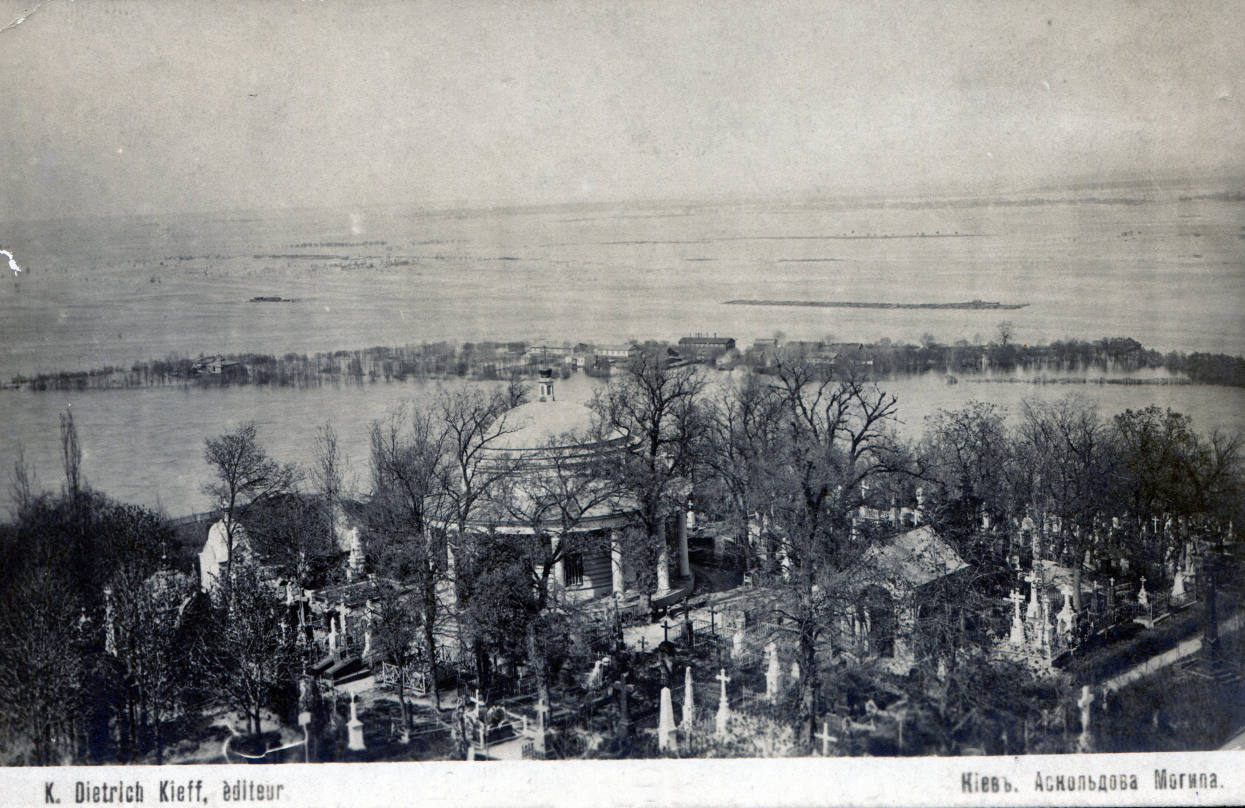
\includegraphics[width=\linewidth]{chast-gorodki/more/amogila1907.jpg}

\textit{1907 год, вид на левый берег с Аскольдовой могилы.}
\end{center}


В книге М. Возняка «Українські перекази»\cite{vozn01} есть невесть откуда переписанное предание о море на Киевщине и Полтавщине, и дескать, приплывавшие кораблями купцы платили киевскому князю десятину, за которую и построили Десятинную церковь. А когда святой Андрей водрузил на здешней горе крест, то море иссякло, но часть его спряталась под горой, и не зря когда Андреевскую церковь строили, то в склоне открылся родник, и чтобы с ним бороться, покупают смолу тряпки. Вот почему на этом храме нет колокола. Чуть ударит, пробьет вода и зальет окрестности. 

Давно залита водой история Киевщины, история всей древней земли вдоль Днепра. Водохранилища навсегда похоронили под собой курганы и давние поселения, затопили луга, уничтожили малые реки, озера, заболотили берега. Горе дому человеческому, горе звериной норе!

Только под Киевским водохранилищем навсегда скрылись селения с именами, от коих веяло стариной – Сорокошичи, Сваромье, восточная часть Козаровичей, Чернин. Иные, где ныне суша по берегам, обезлюдели и стерлись – Теремцы, Новый и Старый Глыбов, Сивки.

А остальные искусственные моря? Гидроэлектростанции дали энергию, платой за нее стала, пожалуй б\'ольшую часть левобережья древнейшего очага цивилизации. Правый же берег неистово пожрали кирпичные заводы да загадили мусорные свалки.
